\chapter{Resultaten}
Het belangrijkste resultaat is natuurlijk de implementatie van het volledige drone systeem.
Uit testen bleek dat de Pozyx tag 110 afstanden per seconde kon bepalen.
Doordat er steeds gebruik wordt gemaakt van vier verschillende ankers, vinden er locatie-updates plaats met een frequentie van \SI{27.5}{\Hz} en verder is de keuze gemaakt om de drone aan te sturen met een frequentie van \SI{10}{\Hz}.\\

Tijdens de proefopstelling is er gebruik gemaakt van vier Pozyx ankers voor de locatiebepaling.
Het doel was dat de drone een op voorhand gedefini\"eerd pad vloog, weergegeven met de witte lijnen op figuur \ref{fig:Opstelling}.
Op figuur \ref{fig:SuccesfullFlight1} staan de \textit{waypoints} en het effectief gevlogen pad tijdens een testvlucht gevisualiseerd.
De \textit{waypoints} (rode plustekens) komen overeen met de hoekpunten van de rechthoek voorgesteld op figuur \ref{fig:Opstelling}.
Rond elk \textit{waypoint} is een cirkel getekend die de grootte van het \textit{waypoint} weergeeft, hier \SI{150}{\mm}.
Wanneer de drone binnen dit bereik valt, heeft hij het \textit{waypoint} bereikt.
De stippellijnen op figurr \ref{fig:SuccesfullFlight1} komen overeen met de tegels van de ruimte, deze zijn \SI{600}{\mm} $\times$ \SI{600}{\mm} groot.
De drone probeert de \textit{waypoints} de doorlopen in wijzerzin, met de linkerbovenhoek als startpunt. 
\begin{figure}[p]
	\centering
	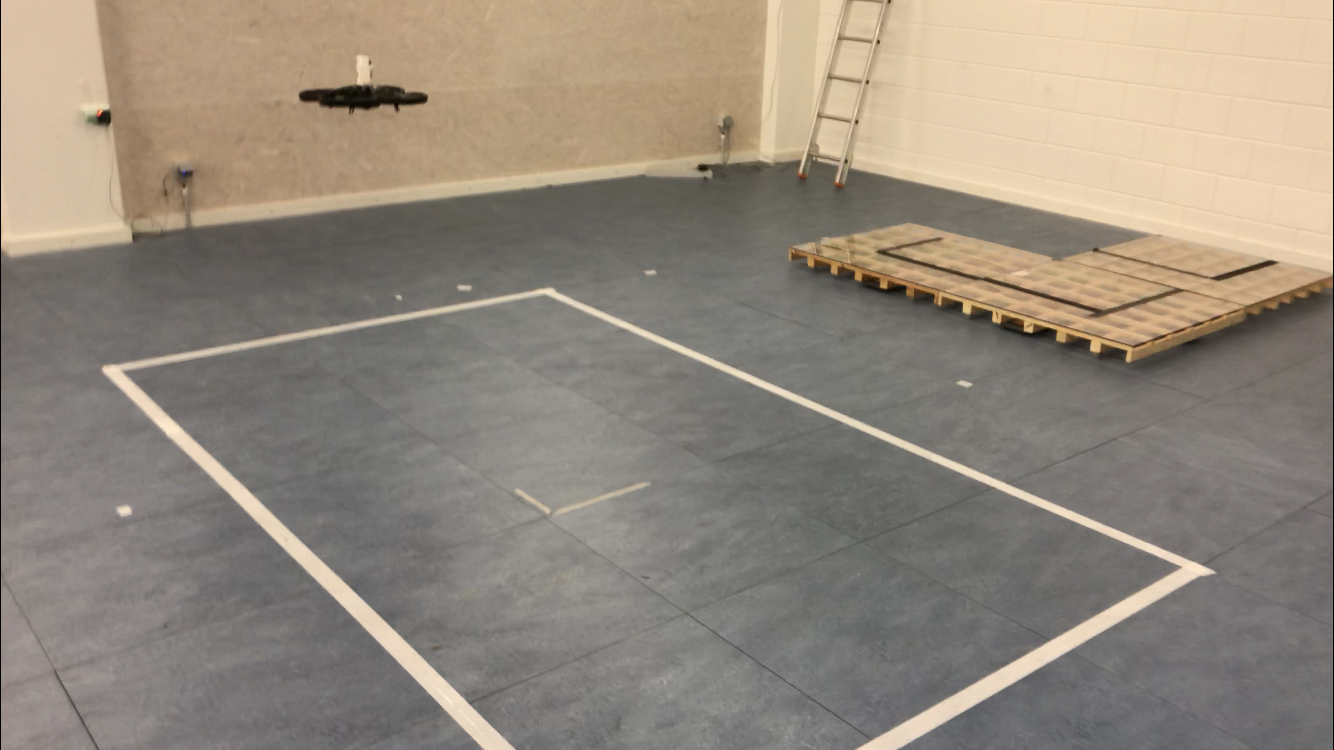
\includegraphics[width=\textwidth]{Opstelling}
	\caption[Opstelling testvluchten]{Testopstelling voor het aansturen van de drone.}
	\label{fig:Opstelling}
\end{figure}

\begin{figure}[p]	
	\centering
	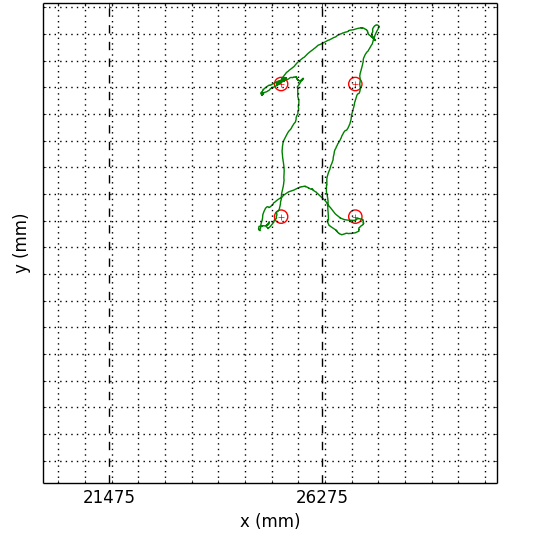
\includegraphics[width=\textwidth]{SuccesfullFlight1}
	\caption[Geslaagde testvlucht]{Geslaagde testvlucht, de drone passeert langs alle waypoints.}
	\label{fig:SuccesfullFlight1}
\end{figure}

\section{Testen} \label{sec:test}
Indien u dit project zelf wil gebruiken of testen, bezoek dan zeker de git repository\footnote{\url{https://github.ugent.be/gartangh/VOP_Voorraadbeheer}} of de website\footnote{\url{https://github.ugent.be/pages/gartangh/VOP_Voorraadbeheer}}.
Hier kan meer informatie gevonden worden over verscheidene onderwerpen, zoals bijvoorbeeld de installatie, MQTT topics en configuratiebestanden.

\section{Problemen} \label{sec:problems}
Een openstaand probleem van het project is dat het verbinden van de off-board controller met twee verschillende netwerken nog niet optimaal verloopt. Vaak wil de applicatie niet verbinden met het netwerk van de drone.\\

Een tekortkoming aan het project is dat de drone momenteel altijd moet opstarten met de voorkant wijzend naar de positieve x-as.
Dit kan manueel niet altijd even nauwkeurig gebeuren waardoor het tweede algoritme vaker moet corrigeren tijdens een vlucht.
Een illustratie van dit probleem is niet voorhanden, maar het kon wel visueel vastgesteld worden.\\

Een mogelijke oplossing voor dit probleem is om de drone op een bepaald punt in de ruimte vast te zetten zodat de lengte van de drone parallel ligt met de x-as, met de voorkant richting het positieve deel.\\
Een andere oplossing is om de drone eerst te calibreren alvorens de vlucht aan te vatten.
Hierbij kan eerst een aantal meter recht vooruit gevlogen worden en vervolgens kan bepaald worden in welke richting de drone gevlogen heeft.
Dit brengt enkele veronderstellingen met zich mee, die haast onmogelijk in werkelijkheid gereproduceerd kunnen worden.
Bijvoorbeeld: de drone moet recht vooruit vliegen, zonder af te wijken door luchtstromingen of te roteren tijdens de vlucht.
Ook is er een relatief grote plaats nodig waar de drone in alle mogelijke richtingen enkele meters kan vliegen.\\

\section{Kosten}
Tot slot geven we een overzicht van de gemaakte kosten binnen dit project.\\
De extra batterij van \SI{1000}{\mA\hour} was nodig om op korte tijd voldoende te kunnen testen.
Zonder die extra batterij zou er telkens een paar uur gewacht moeten worden na een kwartier testen.\\
De eerste LiPo batterijen (van \SI{150}{\mA\hour}) die aangekocht werden bleken niet lang genoeg stroom te kunnen leveren aan de on-board controller. Daarna werd geopteerd voor grotere batterijen van \SI{500}{\mA\hour}.\\
De aankoop van de Adafruit HUZZAH bleek overbodig nadat de controller opgesplitst werd.\\

Een overzicht van alle gemaakte kosten vindt u in tabel \ref{tab:kosten}.\\
Materiaal dat reeds beschikbaar was zoals de Pozyx ankers en tags en de Raspberry Pis is niet in de tabel verwerkt.
\begin{table}[p]
\centering
\begin{tabular}{ |l|r|r|r| } \hline
Product & Prijs (\euro{}) & Aantal & Totaal (\euro{}) \\ [.5ex] \hline \hline
Parrot AR.Drone 2.0 Elite Edition met jungle camo & 116.71 & 1 & 116.71 \\ \hline
Micro USB OTG kabel & 1.32 & 2 & 2.63 \\ \hline
5 LiPo batterijen \SI{150}{\mA\hour} en lader voor controller & 12.46 & 1 & 12.46 \\ \hline
Adafruit HUZZAH & 14.57 & 1 & 14.57 \\ \hline
LiPo batterij \SI{1000}{\mA\hour} voor drone & 34.99 & 1 & 34.99 \\ \hline
2 LiPo batterijen \SI{500}{\mA\hour} en lader voor controller & 35.35 & 1 & 35.35 \\ [.5ex] \hline
Velcro (\SI{1}{\m}) & 0.79 & 1 & 0.79 \\ \hline
\hline
Totaal & & & 217.50 \\ \hline
\end{tabular}
\caption[Kosten]{Verantwoording van gemaakte kosten.}
\label{tab:kosten}
\end{table}